\documentclass{article}

\usepackage[small,compact]{titlesec}
\usepackage[backend=biber]{biblatex}
\usepackage[spanish]{babel}
\usepackage{epsfig}
\usepackage{array}
\usepackage{xfrac}
\usepackage{amsthm}
\usepackage{amsmath}
\usepackage{amssymb}
\usepackage{todonotes}
\usepackage{centernot}
\usepackage{textcomp}
\usepackage{blindtext}
\usepackage{centernot}
\usepackage{wasysym}
\usepackage{siunitx}
\usepackage{minted}
\usepackage[letterpaper]{geometry}
%\usepackage{multicol}
\usepackage{color}
%\usepackage[table]{xcolor}
\usepackage{amsfonts}
\usepackage{mathtools}
\usepackage{multirow}
\usepackage[small,it]{caption}
\usepackage{titling}
\usepackage{graphicx}
\usepackage[short]{optidef}
%\bibliographystyle{plain}
%\bibliographystyle{babplain}
\usepackage{filecontents}
\usepackage{titlesec}
\usepackage[section]{placeins}
\usepackage[hidelinks]{hyperref}
\usepackage{fancyhdr}
\usepackage{cancel}
\usepackage{abstract}
\usepackage{minted}

\sisetup{output-exponent-marker=\textsc{e}}

\captionsetup[table]{name=Table}


%\usepackage[makestderr=true]{pythontex}
%\restartpythontexsession{\thesection}

%\setpythontexoutputdir{./Temp}


\addbibresource{Bibliography.bib}

\pagestyle{fancy}
\usepackage[utf8]{inputenc}
\fancyhf{}
\fancyhead[c]{\textbf{\@title}}
\fancyfoot[c]{\thepage}
\def\Section {\S}

\newcommand\tstrut{\rule{0pt}{2.4ex}}
\newcommand\bstrut{\rule[-1.0ex]{0pt}{0pt}}

\DeclareMathOperator*{\argmax}{arg\,max}
\DeclareMathOperator*{\argmin}{arg\,min}

\setlength{\droptitle}{-4em}
\newcommand{\squishlist}{
 \begin{list}{$\bullet$}
  { \setlength{\itemsep}{0pt}
     \setlength{\parsep}{3pt}
     \setlength{\topsep}{3pt}
     \setlength{\partopsep}{0pt}
     \setlength{\leftmargin}{1.5em}
     \setlength{\labelwidth}{1em}
     \setlength{\labelsep}{0.5em} } }


\newcommand{\squishlisttwo}{
 \begin{list}{$\bullet$}
  { \setlength{\itemsep}{0pt}
    \setlength{\parsep}{0pt}
    \setlength{\topsep}{0pt}
    \setlength{\partopsep}{0pt}
    \setlength{\leftmargin}{2em}
    \setlength{\labelwidth}{1.5em}
    \setlength{\labelsep}{0.5em} } }

\newcommand{\squishend}{
  \end{list}  }
\footskip = 50pt
\setlength{\skip\footins}{10pt}

\newcounter{proofc}
\renewcommand\theproofc{(\arabic{proofc})}
\DeclareRobustCommand\stepproofc{\refstepcounter{proofc}\theproofc}
\newenvironment{twoproof}{\tabular{@{\stepproofc}c|l}}{\endtabular}

\usemintedstyle{tango}
 %% The usual stuff that sits
 %% between \documentclass
 %%    and \begin{document}

%\hypersetup{
%    bookmarks= \quadtrue,         % show bookmarks bar?
%    unicode= \quadfalse,          % non-Latin characters in Acrobat’s bookmarks
%    pdftoolbar= \quadtrue,        % show Acrobat’s toolbar?
%    pdfmenubar= \quadtrue,        % show Acrobat’s menu?
%    pdffitwindow= \quadfalse,     % window fit to page when opened
%    pdfstartview= \quad{FitH},    % fits the width of the page to the window
%    pdftitle= \quad{My title},    % title
%    pdfauthor= \quad{Author},     % author
%    pdfsubject= \quad{Subject},   % subject of the document
%    pdfcreator= \quad{Creator},   % creator of the document
%    pdfproducer= \quad{Producer}, % producer of the document
%    pdfkeywords= \quad{keyword1} {key2} {key3}, % list of keywords
%    pdfnewwindow= \quadtrue,      % links in new window
%    colorlinks= \quadfalse,       % false: boxed links; true: colored links
%    linkcolor= \quadred,          % color of internal links (change box color with linkbordercolor)
%    citecolor= \quadgreen,        % color of links to bibliography
%    filecolor= \quadmagenta,      % color of file links
%    urlcolor= \quadcyan           % color of external links
%}

%\addbibresource{References.bib}


\begin{document}
 %\thispagestyle{plain}
 \def\maketitle{%\twocolumn[%
 \thispagestyle{plain}
 \vspace{-10ex}
 \hrule
 \bigskip
 \begin{center}
 {\Large{\textbf{\@title}}}
 \end{center}
 \bigskip
 \hrule

 \bigskip

 \begin{flushleft}
 \textbf{\normalsize{Edgar Andr\'{e}s Margffoy Tuay}} \hfill 201412566
 \\
 \vspace{5pt}
 Universidad de los Andes \hfill Concurrency, Parallelism and Distribution
 \\
 \vspace{5pt}
\hfill \today \\ 
 \end{flushleft}
 %\hspace{265.2pt}
 %\bigskip
 %\bigskip
 }
\def\title#1{\def\@title{#1}}
\title{\textit{Conway's Game of Life}}



% \squishlist    %% \begin{itemize}
%\item First item
%%\item Second item
%%\squishend     %% \end{itemize}
 %% The rest of the paper (with no maketitle)
\maketitle

\section{Implementation Details}
Due to its local behaviour, the Conway's Game of Life can be approached as a parallel problem, on which, each update to each individual cell does not depend on the update result of the other cells. Moreover, a Game of Life board can be seen as a collection of sub-boards that also are instances of the Game of Life, and therefore it represents a parallel recursive function that can be implemented via Fork-Foin.

Formally, given a board of size $m \times n$, we take four sub-boards of size $\sfrac{m}{2} \times \sfrac{n}{2}$ and apply recursively the Life game board partition, until the resulting board dimensions are $m_c \times n_c$, with $m_c$ and $n_c$, being the cutoff height and width, respectively. Then the B3/S23 rule is applied over the cutoff board. When all four processes finish, the parent process is on charge of merging all the subarrays into a single board. An important note about this process, is that cells that lie on a board boundary, depend on the state of cells that are across the boundary on other boards. To overcome this issue, for each sub-board, the partition implementation takes into account ghost cells that keep track of the cells that are on other boards, but are not to be updated after applying the rules to the sub-board. Figure \ref{Fig:F1} depicts the process. To run an example board, please execute \texttt{LifeCLI.example} on the \texttt{iex} interpreter.

\begin{figure*}[!htbp]
	 \centering
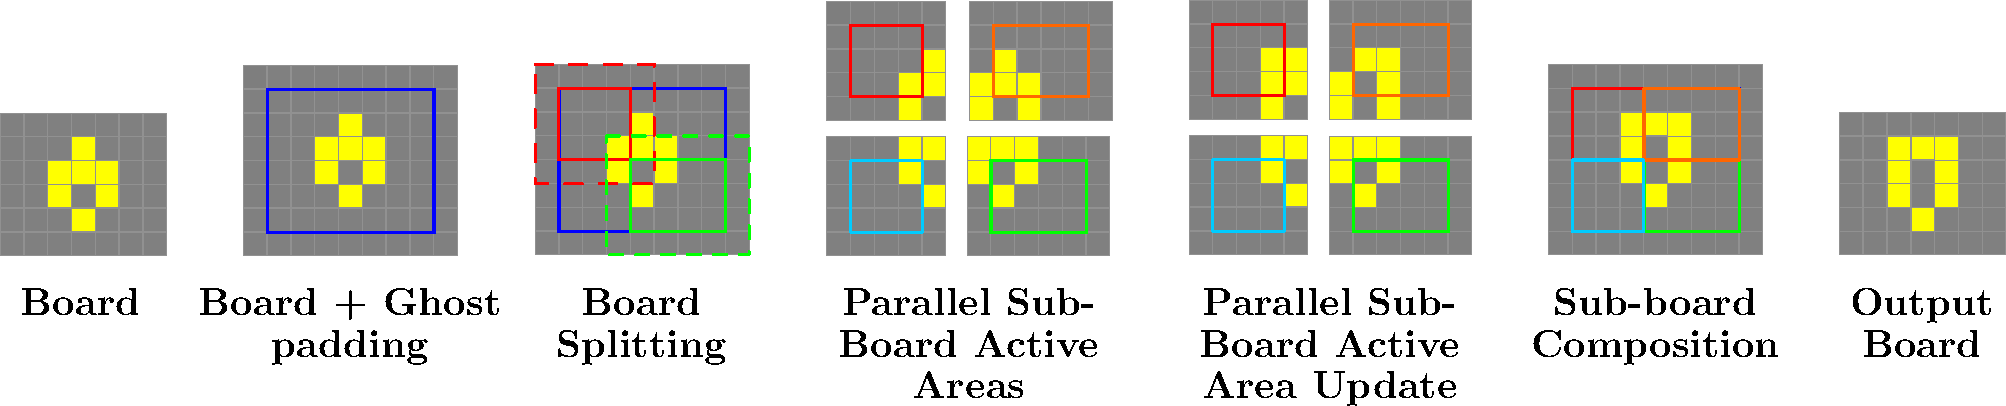
\epsfig{file=./Assets/Fork.pdf,width=1.0\linewidth,clip=}
\caption{Parallel Conway's Game of Life: First, given a board, padding is added such that boundary cells can be updated. Then, the active area is split into four subarrays and assigned to a parallel process, each one of them contain additional columns and rows that allow to update their corresponding boundary cells. When the array dimensions are lesser or equal to the cutoff value, the active area cells are updated in parallel. Finally, the parent process assembles the final board using the resulting active areas of each worker. }
\label{Fig:F1}
\end{figure*}



\subsection{Parallel Complexity}
Due to the independence between concurrent cell updates, and given enough resources, the process can be parallelized up to $mn$ processors. Given that the work $T_1$ elapsed by a single processor corresponds to $\mathcal{O}(mn)$, the complexity of the parallel work $T_P$ corresponds to $\mathcal{O}(1)$. With respect to the span of the parallel process $T_\infty$, this measure is bounded by the costs of splitting and merging arrays, which in the worst case correspond to $\mathcal{O}(m + n)$ (assuming constant array access cost and constant array merging time). Thus, the total complexity for the parallel version of Conway's Game of Life corresponds to $\mathcal{O}(m + n)$.  

\squishlist
\item Span: $\mathcal{O}(m + n)$
\item Work: $\mathcal{O}(1)$
\squishend   

%\subsection{Could it be implemented on Elixir}
%As all lists and variables (Including parallel collections) are immutable on Elixir, the Scala implementation cannot be ported as-is, due to its reliance on memory manipulations (In-place modifications and memory copying) for optimal running time. Thus, there would be no time execution reduction if it was to be implemented on Elixir, \textit{i.e.,} Listing \ref{lst:L2}. 
%\begin{alignat}{2}
%&\tilde{H} = \begin{bmatrix}
%\mathbf{A} & \mathbf{t} \\
%\mathbf{u}^{T} & \alpha
%\end{bmatrix} & \quad   \label{eq:e1}
%\end{alignat}



%\begin{figure}[!htbp]
%\centering
%\includegraphics[scale=0.3]{./Assets/1.png}
%\caption{Traza de Wireshark que presenta la emisión y recepción de paquetes ICMP enviados a un conjunto de %clientes presentes en la misma red.}
%\end{figure}


%\section{Diseño de filtros ideales}

%\begin{alignat}{2}
%h &= \begin{bmatrix}
%1 & 1 & 1 \\
%1 & 1 & 1 \\
%1 & 1 & 1 
%\end{bmatrix} \label{eq:e6}
%\end{alignat}


% \begin{equation}
% \begin{aligned}
% f ~:~ &\mathbb{R} &\longrightarrow ~ &\mathbb{R} \label{eq:e6} \\
%     &t &\longmapsto ~ &f(t)
% \end{aligned}
% \end{equation}
% \begin{equation}
% \begin{aligned}
% x ~:~ &\mathbb{Z} &\longrightarrow ~ &\mathbb{R} \label{eq:e7} \\
%     &n &\longmapsto ~ &x[n]
% \end{aligned}
% \end{equation}



% \begin{figure*}[!htbp]
% \centering
% \epsfig{file=./Assets/Discrete.pdf,width=1.0\linewidth,clip=}
% \caption{Ejemplos de señales discretas}
% \label{Fig:F3}
% \end{figure*}




%\bibliography{biblios} \nocite{*}
%\newpage
%\nocite{*}
%printbibliography



%\newcounter{proofc}
%\renewcommand\theproofc{(\arabic{proofc})}
%\DeclareRobustCommand\stepproofc{\refstepcounter{proofc}\theproofc}
%\newenvironment{twoproof}{\tabular{@{\stepproofc}c|l}}{\endtabular}


\end{document}